\documentclass[a4paper,12pt,oneside]{article}
\usepackage{graphicx}
\usepackage{color}
\usepackage{graphicx}
%% Front Page 
\title{\bf \LARGE {Computer Networks Lab(EEP 703)\\
\\[0.5cm]  Assignment 10: Generating and analyzing network traffic}}
\author{Name : Harshit Kumar Gupta \\Entry Number : 2013EET2369
\\[0.5cm]Computer Technology \\Department of Electrical Engineering
\\[0.5cm]
\includegraphics[scale=.5]{./IITD.png}
\\[2cm]\bf \LARGE{Indian Institute of Technology Delhi}}
\date{February 5, 2014}

\newpage
\begin{document}
\maketitle
\newpage
%% Contents
\tableofcontents






%% Problem State
\newpage

 \section{Problem Statement:}


\noindent{In this assignment, we will learn to capture traffic on our system and analyze it
using Wireshark tool.}\\[.25cm]
\begin{enumerate}
\item Accomplish the following tasks:
\item Using wireshark, observe normal network traffic. Can you separately see TCP/IP traffic, 
IPX traffic and NETBEUI traffic? What is the meaning of these different types of traffic? 
\item Using wireshark, observe normal network traffic. Can you separately see TCP/IP traffic, 
IPX traffic and NETBEUI traffic? What is the meaning of these different types of traffic? 
\item Using Ostinato, configure and generate connectionless and connection­oriented packet services 
in your system. Generate such traffic for following two cases: 
\item CASE 1: Low transmission rate with small packet length  
\item CASE 2: High transmission rate with large packet length.
\item Find throughput for both the cases for each packet service (connectionless and 
connection­oriented) and comment on what you observe.
\end{enumerate}
Perform following and comment on the response you get:
\begin{enumerate}
\item Increase the rate at which ostinato is sending data. As you do so, observe that you seem 
to be able to send at whatever data rate you want. This is obviously wrong ­ what could 
be happening ?  

\item If you were given the task of developing a ostinato like generator , how would you start 
and go about it ? How would you ‘test’ your generator ?
\end{enumerate}


\newpage

\section {Abstract}

In this experiment we will create analyze our present network using a network tool called WIRESHARK.
We would learn how to recognise the network internet protocol addresses (IP) of various websites and to analye the network and various packets sent to/from the website using 
wireshark software.We also analyse the packets sent by the website and learn about various terminologies assocaited with it like various headers
,IP versions etc.

\newpage


\section{Execution Directive}  
Type the following commands on the terminal window in order to perform the given task.
\begin{enumerate}
 \item Open wireshark as root user.
 \item Open interface ethernet to capture the network  
 \item Start the interface and open the website whose analysis is to be seen.
 \item Open Ostinato and the select a port for transmission.
 \item Modify the properties of the transmission and start the transmission
 \item Start capture.
 \item View the capture ion wireshark.
 \end{enumerate}
\begin{center}
 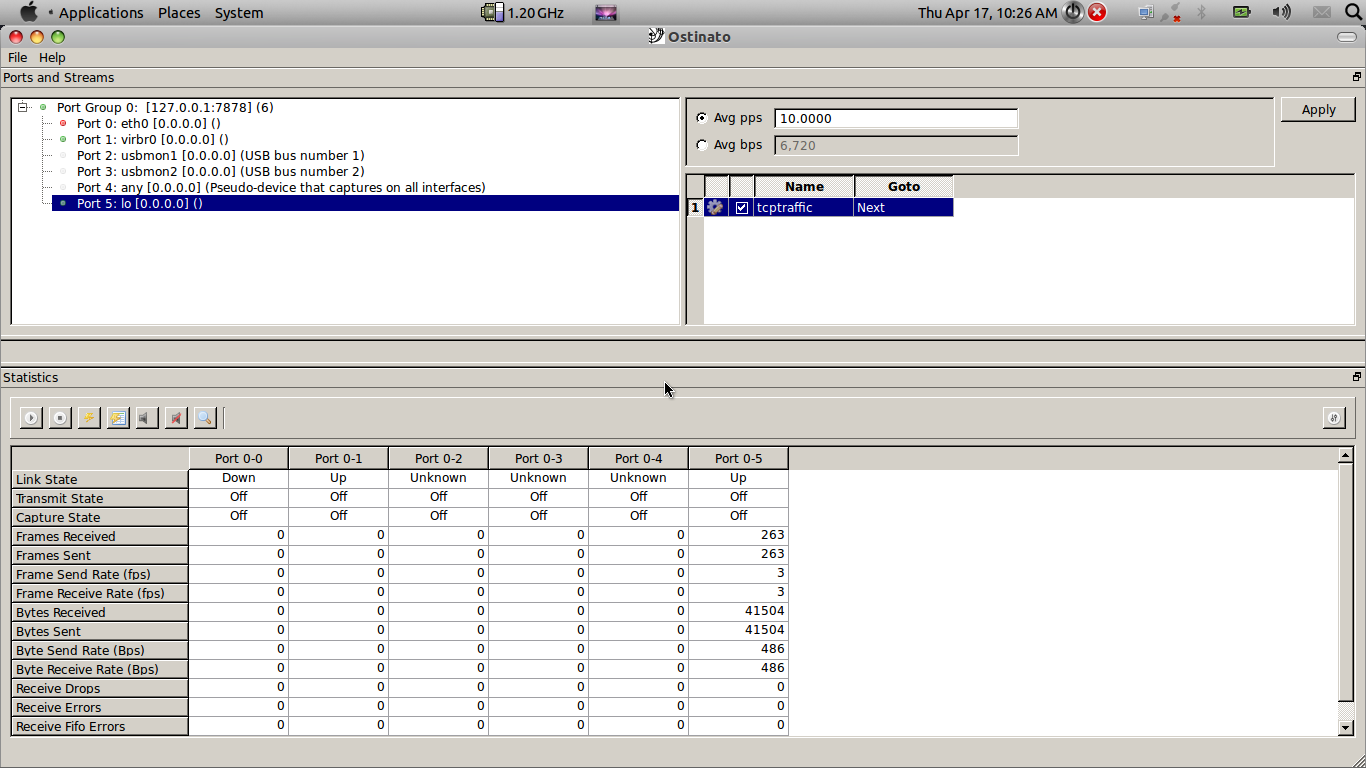
\includegraphics[width=13 cm,height=12 cm]{./tcptraffic.png}
Generation of TCP traffic
\end{center}
\begin{center}
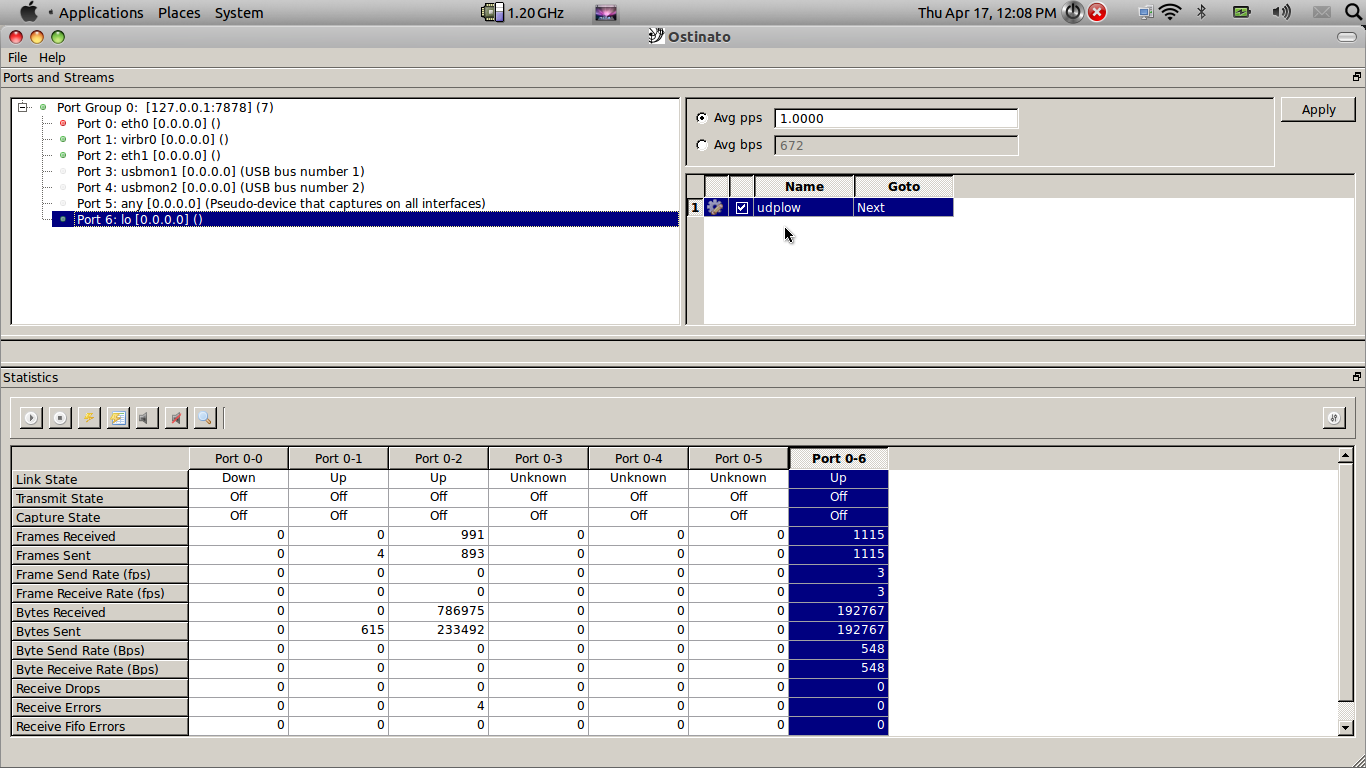
\includegraphics[width=13 cm,height=12 cm]{./udptraffic.png}
 Generation of UDP traffic
\end{center}
 \newpage


\section{Result And Discussions}
\begin{enumerate}
\item Problem Statement 1
\begin{enumerate}
\item Yes we can see the the TCP/IP,IPX and NETBEUI traffic in the wireshark network capture.IPX/SPX and TCP/IP are both operational on
OSI model as layer 3 and layer 4 network protocols.IPX is basically well suited for local networks whereas TCP/IP is mainly used for interenet and WLANs.
Their comparison along with a brief description of the NETBIOS protocol is given below-



 \item  Transmission Control Protocol / Internet Protocol (TCP/IP) :: TCP/IP (Transmission Control Protocol/Internet Protocol) is the basic communication language or protocol of the Internet. It can also be used as a communications protocol in a private network (either an intranet or an extranet). When you are set up with direct access to the Internet, your computer is provided with a copy of the TCP/IP program just as every other computer that you may send messages to or get information from also has a copy of TCP/IP.


\item TCP/IP is a two-layer program. The higher layer, Transmission Control Protocol,
manages the assembling of a message or file into smaller packets that are transmitted over the Internet
and received by a TCP layer that reassembles the packets into the original message.
\item The lower layer, Internet Protocol, handles the address part of each packet so that it gets to the right destination. Each gateway computer on the network checks this address to see where to forward the message. Even though some packets from the same message are routed differently than others, they'll be reassembled at the destination.
\end{enumerate}
\begin{center}
 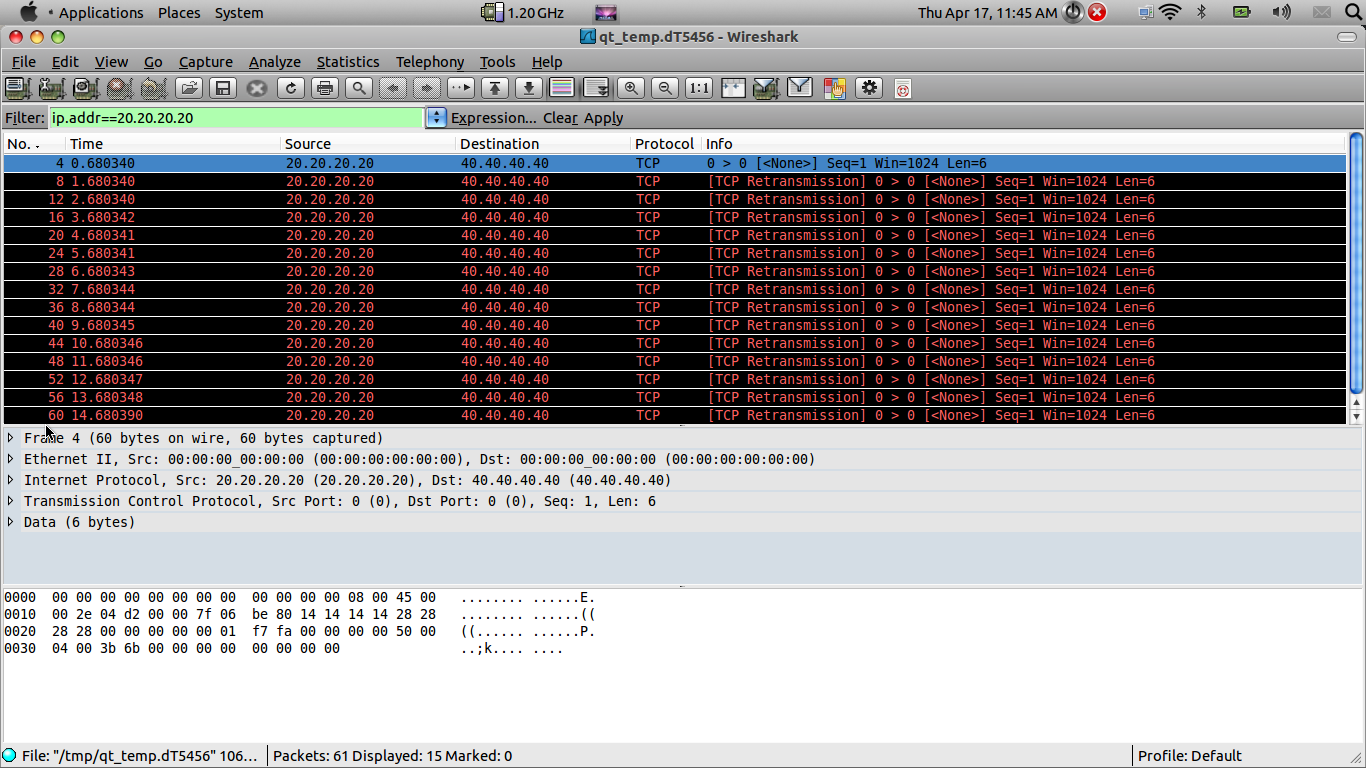
\includegraphics[width=13 cm,height=12 cm]{./tcp.png}
\end{center}
\begin{center}
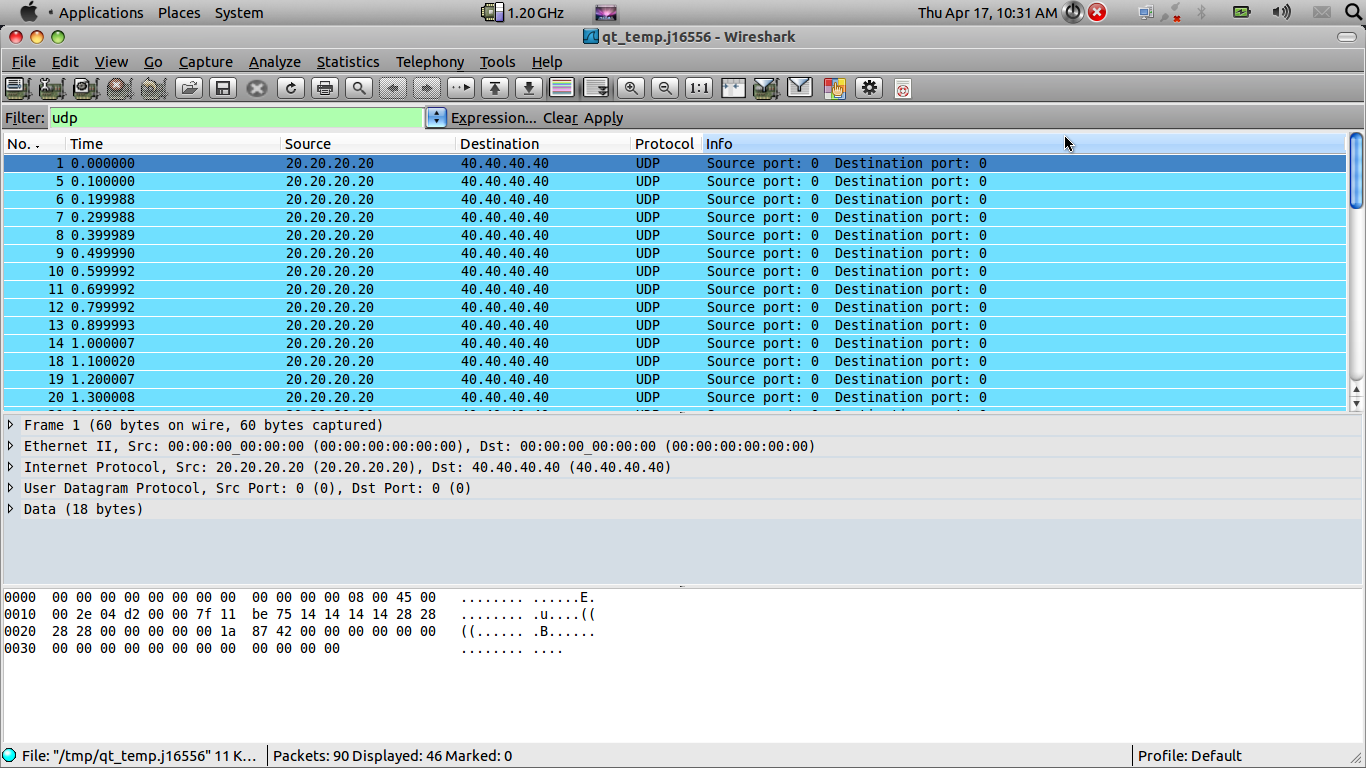
\includegraphics[width=13 cm,height=12 cm]{./udp.png}
 
\end{center}

\newpage
\begin{enumerate}
\item Internetwork Packet eXchange (IPX) :: Internetwork Packet Exchange (IPX) is the OSI-model Network layer protocol in the IPX/SPX protocol stack.



\item A big advantage of IPX is an easy configuration of the client computers. 
\item However, IPX did not scale enough for large networks such as the internet[1] and as such, IPX usage decreased as the boom of the Internet made TCP/IP nearly universal. Computers and networks can run multiple network protocols,
so almost all IPX sites will be running TCP/IP as well to allow for Internet connectivity.[
\end{enumerate}
\begin{center}
 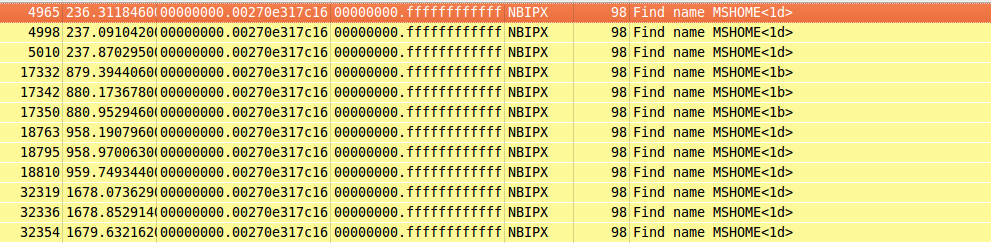
\includegraphics[width=13 cm,height=12 cm]{./ipx.png}
\end{center}
\newpage
\begin{enumerate}
\item  Network Basic Input/Output System (NETBEUI/NETBIOS} : 
t provides services related to the session layer of the OSI model allowing applications on separate computers to communicate over a local area network. 

\item As strictly an API, NetBIOS is not a networking protocol. 
\item NetBios can work over IPX/SPX using the NetBIOS Frames (NBF) and IPX/SPX (NBX) protocols. In modern networks, NetBIOS normally runs over TCP/IP via the NetBIOS over TCP/IP (NBT) protocol. 
\end{enumerate}

\begin{center}
 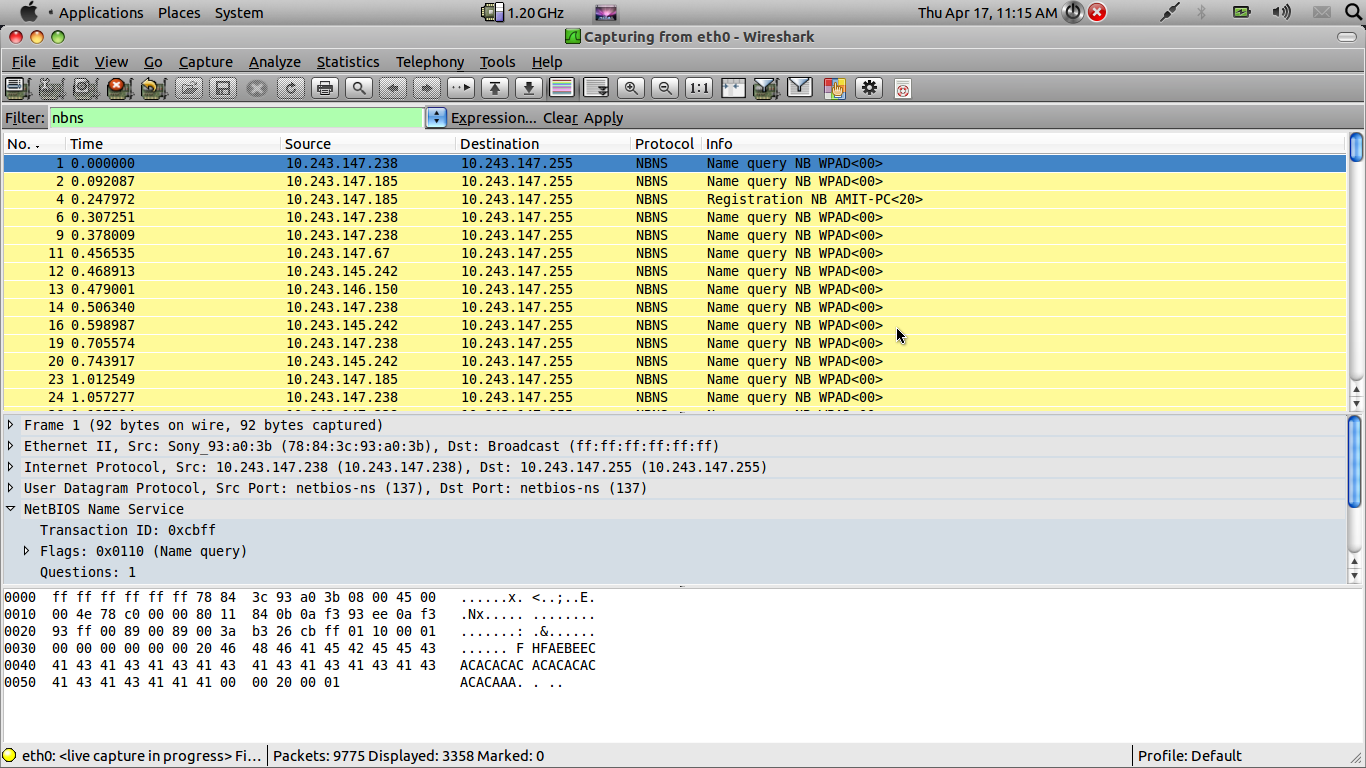
\includegraphics[width=13 cm,height=12 cm]{./nbns.png}
\end{center}
\end{enumerate}
\newpage
\begin{enumerate}
\item The Dynamic Host Configuration Protocol (DHCP) is a standardized networking protocol used on Internet Protocol (IP) networks 
for dynamically distributing network configuration parameters, such as IP addresses for interfaces and services.
\item With DHCP computers request IP addresses and networking parameters automatically from a DHCP server, reducing the need 
for a network administrator or a user from having to configure these settings manually.
\item Yes we can see DHCP packets in the Wireshark capture.

\end{enumerate}
 

\begin{center}
 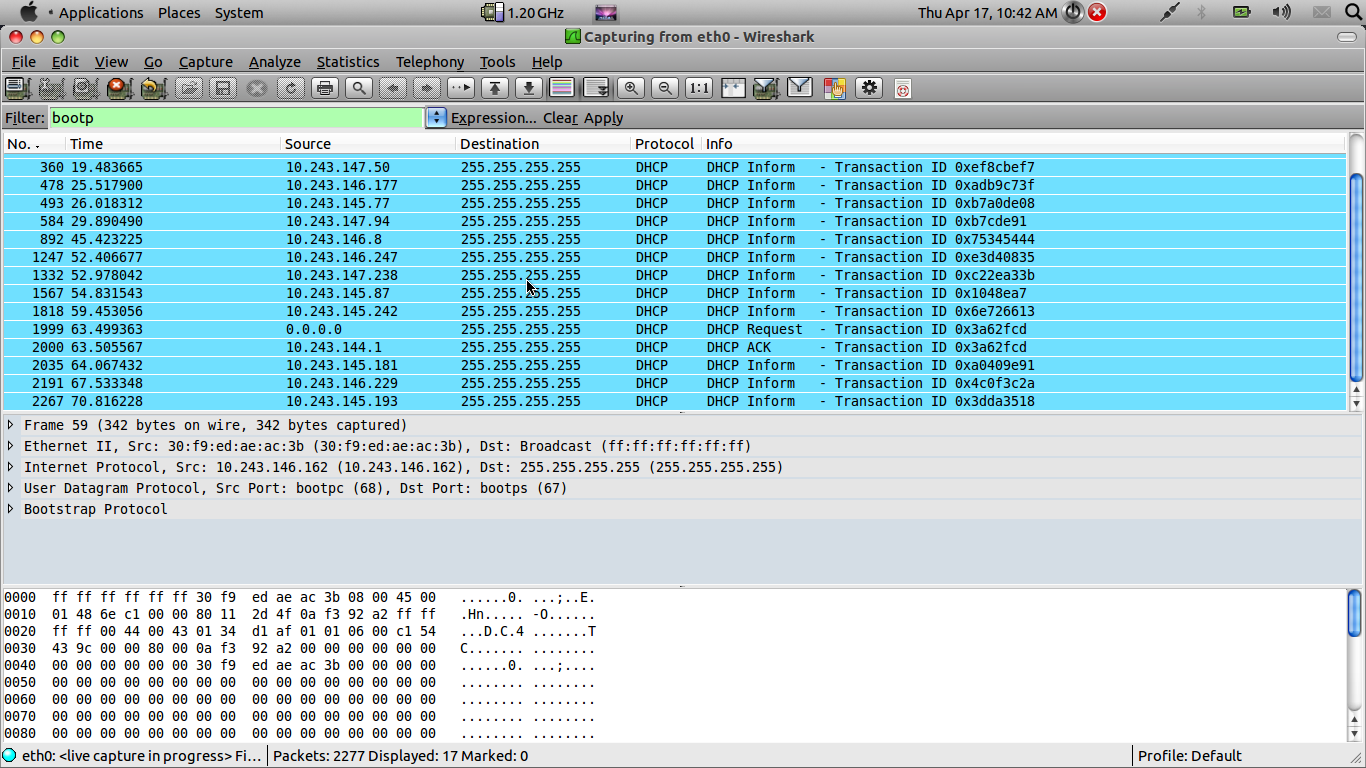
\includegraphics[width=13 cm,height=12 cm]{./dhcp.png}
\end{center}


\begin{enumerate}
\item MECHANISM ::
\item The client broadcasts messages on the network subnet using the destination address 255.255.255.255 or the specific subnet broadcast address.
\item A DHCP client may also request its last-known IP address.
\item If the client remains connected to the same network, the server may grant the request. 
\item Otherwise, it depends whether the server is set up as authoritative or not. 
\item An authoritative server denies the request, causing the client issue a new request. 

\end{enumerate}

\begin{center}
 
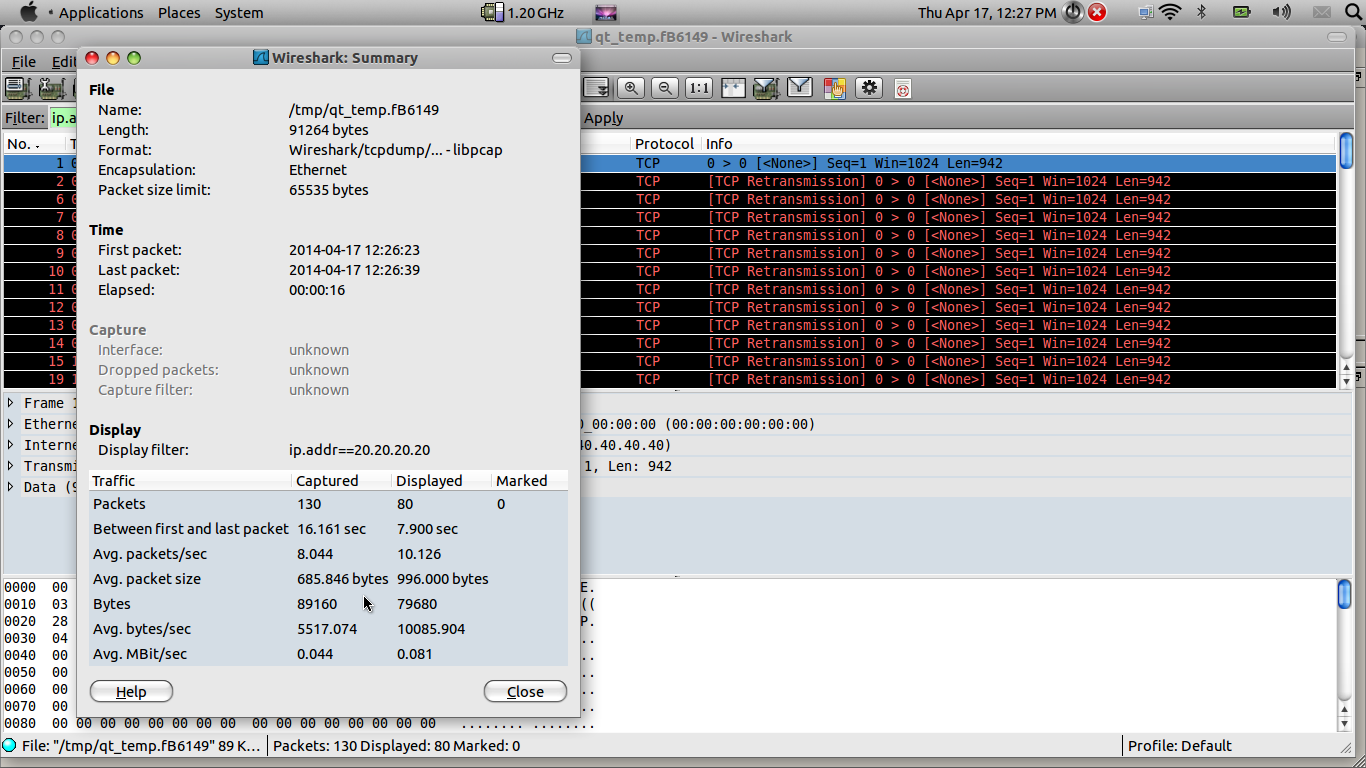
\includegraphics[width=13 cm,height=12 cm]{./tcphigh.png}
 High Transmission rate High packet size :: TCP 
\end{center}
 
\begin{center}
 
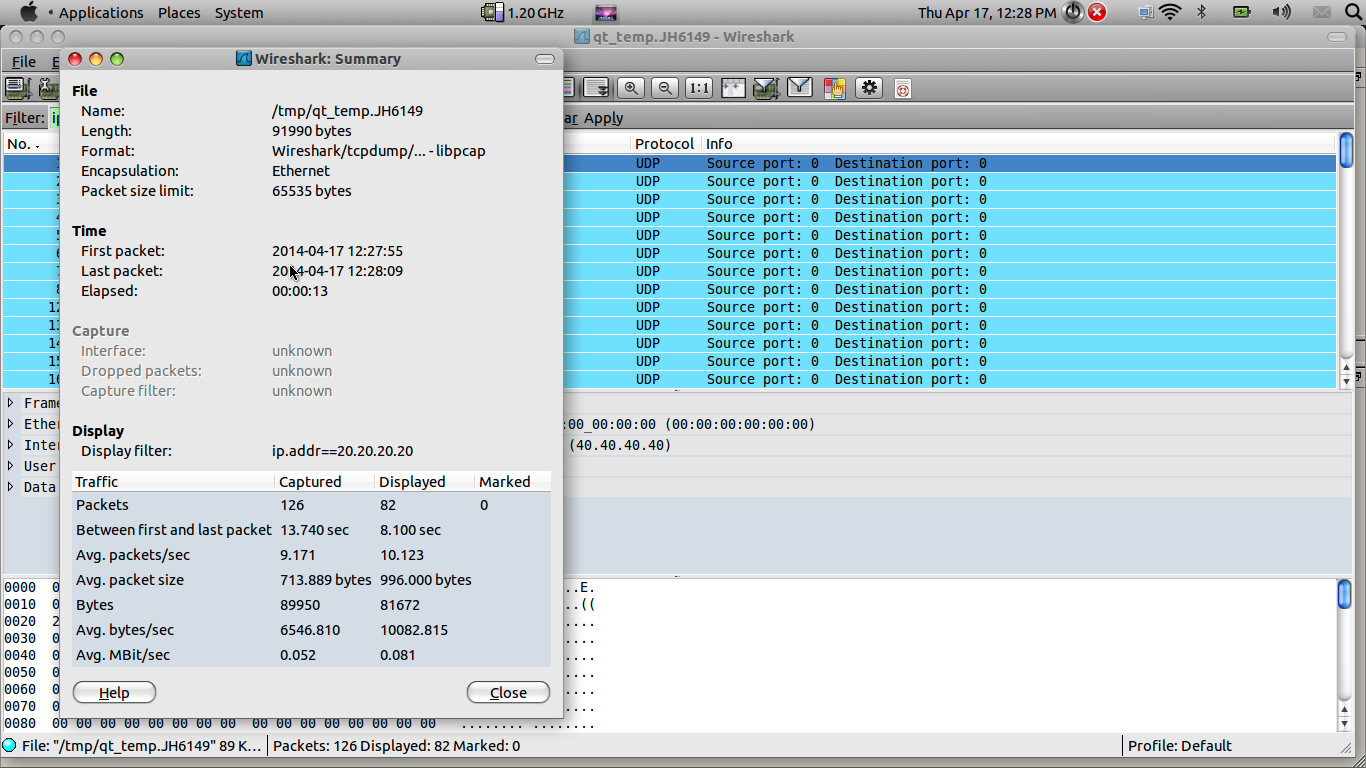
\includegraphics[width=13 cm,height=12 cm]{./udphigh.png}
 High Transmission rate High packet size :: UDP  
\end{center}

\begin{center}
 
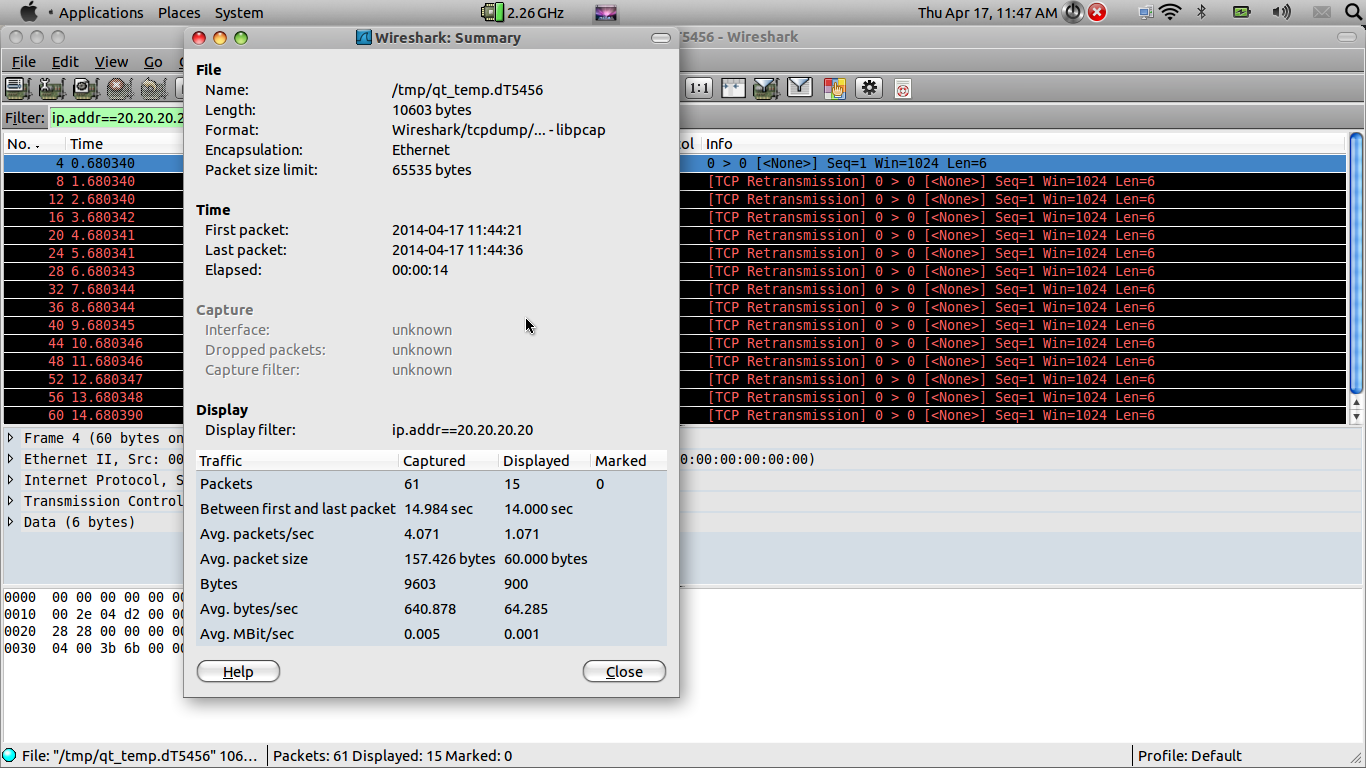
\includegraphics[width=13 cm,height=12 cm]{./tcplow.png}
 Low Transmission rate Low packet size :: TCP  
\end{center}
 
\begin{center}
 
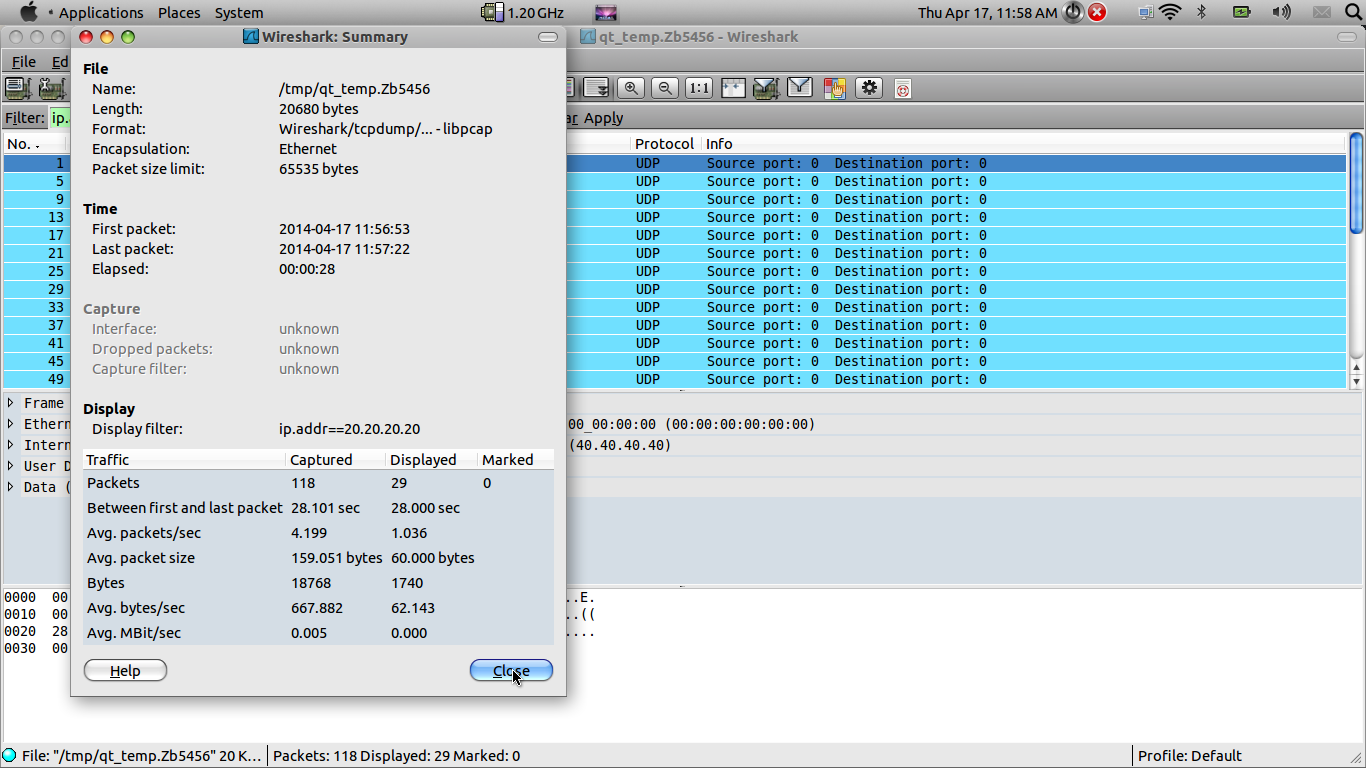
\includegraphics[width=13 cm,height=12 cm]{./udplow.png}
 Low Transmission rate Low packet size :: UDP 
\end{center}



 
 

\end {document}
